\documentclass[11pt,twoside,twocolumn]{usgsreport}
\usepackage{usgsfonts}
\usepackage{usgsgeo}
\usepackage{usgsreporta}
\usepackage{graphicx}
\usepackage{float}
\graphicspath{{./figures/}}

\renewcommand{\cooperator}
{the \textusgs\ Office of Groundwater}
\renewcommand{\reporttitle}
{MODPATH Shapefile Exporter---Quick Start Guide}
\renewcommand{\coverphoto}{modpath_cover.png}
\renewcommand{\reportseries}{January 5, 2018}
\renewcommand{\reportnumber}{}
\renewcommand{\reportyear}{2018}
\renewcommand{\covercolor}{
  \definecolor{coverpagecolor}{RGB}{255, 255, 255}
  \pagecolor{coverpagecolor}
}
\definecolor{coverbar}{RGB}{0, 47, 87}
\renewcommand{\bannercolor}{\color{coverbar}}

\begin{document}
\makefrontcover
\makefrontmatterabv
\pagestyle{body}
\SECTION{Introduction}
The MODPATH Shapefile Exporter utility is a Microsoft Windows application for converting MODPATH-7 endpoint, pathline, and timeseries particle coordinate output files to ESRI shapefiles that can be used to display attribute-tagged points and lines in graphic display applications such as the ESRI ArcMap and ArcScene applications.
\SECTION{Running MODPATH Shapefile Exporter}
MODPATH Shapefile Exporter consists of a Microsoft Windows executable file and several dynamically-linked library (DLL) files. No special installation is required. The application should run on any computer running Microsoft Windows 7 SP1 or newer. The files can be placed anywhere provided that the executable file and all the DLL files are located in the same directory.

To run MODPATH Shapefile Exporter, double click on the executable file in Windows explorer and the application window will appear. It also may be convenient to create a desktop shortcut to the executable file that can be used to launch the program.
\begin{figure}[H]
 \centering
  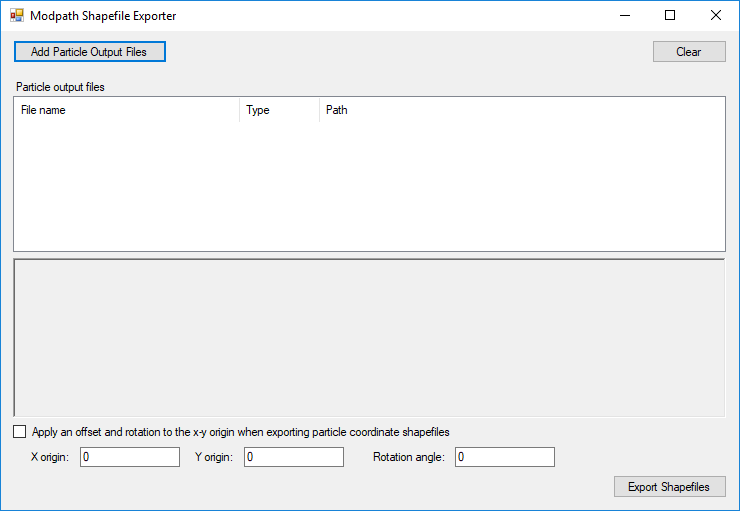
\includegraphics[width=\linewidth]{mf_shp_ex_1.PNG}
\end{figure}

Click the "Add particle output files" button and browse to a folder containing a MODPATH simulation to select a MODPATH-7 simulation file (MPSIM file). A list of the particle coordinate output files specified in the simulation file will appear in the particle output files list.

\begin{figure}[H]
  \centering
  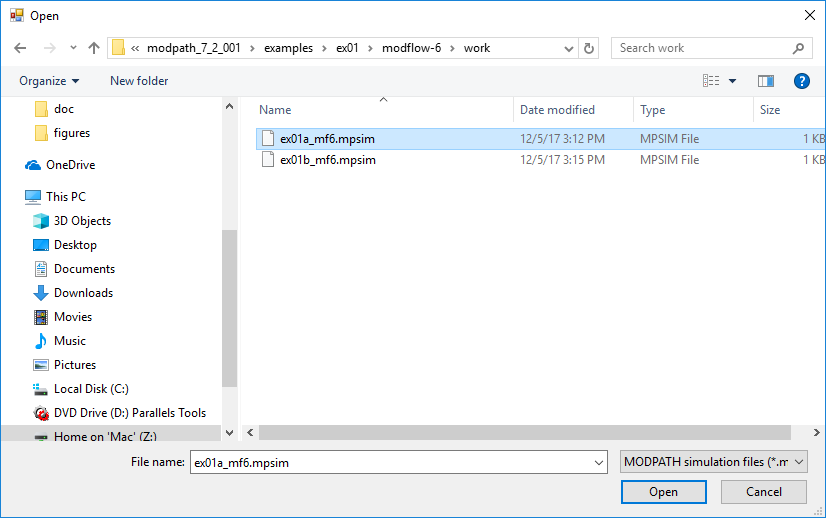
\includegraphics[width=\linewidth]{mf_shp_ex_2.PNG}
  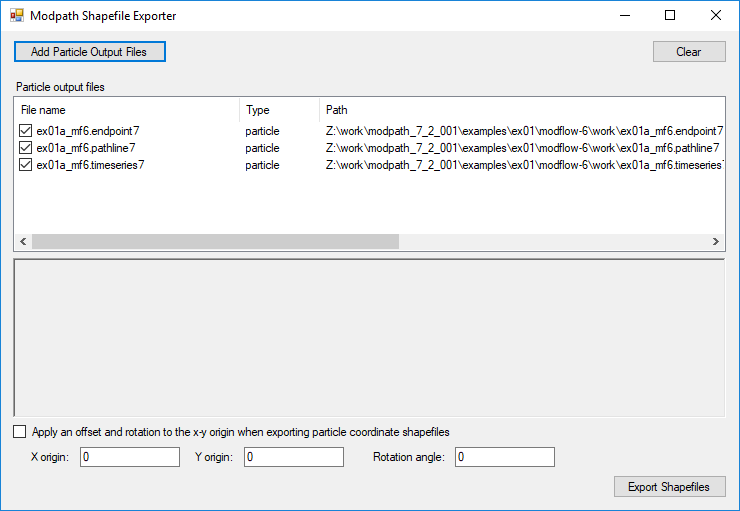
\includegraphics[width=\linewidth]{mf_shp_ex_3.PNG}
\end{figure}

Check the boxes for the files that you want to export as shapefiles and click the "Export Shapefiles" button to create the shapefiles. The status of the export process is summarize3d in the text box.

\begin{figure}[H]
 \centering
  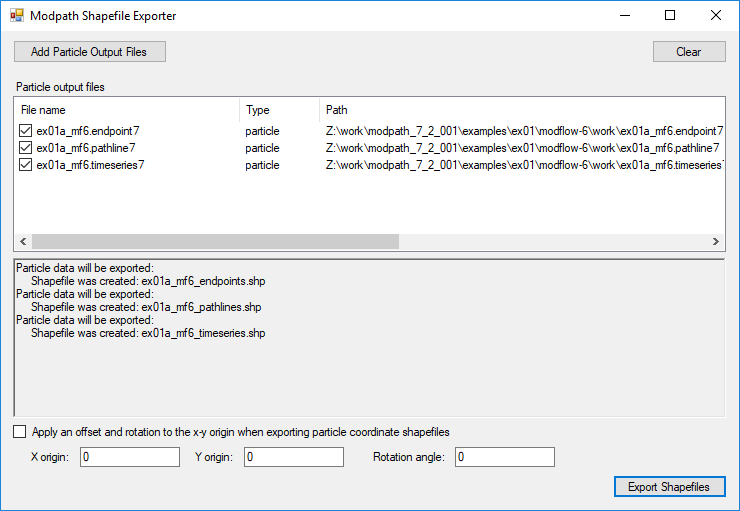
\includegraphics[width=\linewidth]{mf_shp_ex_4.PNG}
\end{figure}

MODPATH generates particle output files based on a coordinate system defined relative to the grid that has an origin of (0, 0) located in the lower left corner of the MODFLOW grid or the quadpatch base grid. An option is provided to specify spatial transformation data (rotation angle, and x and y origin offsets) to generate particle shapefiles that conform to a spatially-transformed grid. Check the box to apply the spatial transformation data and then specify the rotation angle and offset values. 

\SECTION{Endpoint Shapefile}
For forward tracking simulations, the point shapes correspond to the final particle locations. For backward tracking simulations, the point shapes correspond to the final particle locations. The shapefile attributes are:

\begin{description}
  \item[$\bullet$ ] SeqNumber -- MODPATH simulation sequence number
  \item[$\bullet$ ] Group -- particle group number
  \item[$\bullet$ ] ParticleID -- particle ID number within the particle group
  \item[$\bullet$ ] InitLayer -- initial model layer
  \item[$\bullet$ ] FinalLayer -- final model layer
  \item[$\bullet$ ] InitCell -- initial cell number
  \item[$\bullet$ ] FinalCell -- final cell number
  \item[$\bullet$ ] InitTime -- initial tracking time
  \item[$\bullet$ ] FinalTime -- final tracking time
  \item[$\bullet$ ] TravelTime -- particle travel time (FinalTime - InitTime)
  \item[$\bullet$ ] InitZone -- zone number of initial cell
  \item[$\bullet$ ] FinalZone -- zone number of final cell
  \item[$\bullet$ ] Status -- status code of the particle at the end of the simulation
\end{description}

\SECTION{Pathline Shapefile}
The shapefile attributes are:

\begin{description}
  \item[$\bullet$ ] SeqNumber -- MODPATH simulation sequence number
  \item[$\bullet$ ] Group -- particle group number
  \item[$\bullet$ ] ParticleID -- particle ID number within the particle group
  \item[$\bullet$ ] FirstTime -- initial tracking time
  \item[$\bullet$ ] LastTime -- final tracking time
  \item[$\bullet$ ] InitZone -- zone number of initial cell
  \item[$\bullet$ ] FinalZone -- zone number of final cell
\end{description}

\SECTION{Timeseries Shapefile}
Insert paragraphs here

\begin{description}
  \item[$\bullet$ ] SeqNumber -- MODPATH simulation sequence number
  \item[$\bullet$ ] Group -- particle group number
  \item[$\bullet$ ] ParticleID -- particle ID number within the particle group
  \item[$\bullet$ ] TimePoint -- time point index
  \item[$\bullet$ ] TimeStep -- cumulative MODFLOW time step number
  \item[$\bullet$ ] Time -- tracking time
  \item[$\bullet$ ] TravelTime -- travel time (tracking time - initial time). The initial time is obtained from the endpoint file.
  \item[$\bullet$ ] Layer -- model layer
  \item[$\bullet$ ] InitZone -- zone number of initial cell
  \item[$\bullet$ ] FinalZone -- zone number of final cell
  \item[$\bullet$ ] Elevation -- elevation of particle coordinate
\end{description}

\vspace*{\fill}
\clearpage
\pagestyle{backofreport}
\makebackcover
\end{document}